\documentclass[10pt]{beamer}
\usetheme[
%%% options passed to the outer theme
%    hidetitle,           % hide the (short) title in the sidebar
%    hideauthor,          % hide the (short) author in the sidebar
%    hideinstitute,       % hide the (short) institute in the bottom of the sidebar
%    shownavsym,          % show the navigation symbols
%    width=2cm,           % width of the sidebar (default is 2 cm)
%    hideothersubsections,% hide all subsections but the subsections in the current section
%    hideallsubsections,  % hide all subsections
%    left                % right of left position of sidebar (default is right)
  ]{Aalborg}
  
% If you want to change the colors of the various elements in the theme, edit and uncomment the following lines
% Change the bar and sidebar colors:
%\setbeamercolor{Aalborg}{fg=red!20,bg=red}
%\setbeamercolor{sidebar}{bg=red!20}
% Change the color of the structural elements:
%\setbeamercolor{structure}{fg=red}
% Change the frame title text color:
%\setbeamercolor{frametitle}{fg=blue}
% Change the normal text color background:
%\setbeamercolor{normal text}{bg=gray!10}
% ... and you can of course change a lot more - see the beamer user manual.

\usepackage[utf8]{inputenc}
\usepackage[spanish]{babel}
\usepackage[T1]{fontenc}
% Or whatever. Note that the encoding and the font should match. If T1
% does not look nice, try deleting the line with the fontenc.

%\usepackage[table,xcdraw]{xcolor}
\usepackage{helvet}
\usepackage{graphicx}
\usepackage{tikz}
\usetikzlibrary{shapes,arrows,positioning}

%\usepackage{minted}
\usepackage{listings}
\usepackage{color}
\definecolor{codegreen}{rgb}{0,0.6,0}
\definecolor{codegray}{rgb}{0.5,0.5,0.5}
\definecolor{codepurple}{rgb}{0.58,0,0.82}
\definecolor{backcolour}{rgb}{0.95,0.95,0.92}
 
\lstdefinestyle{mystyle}{
    backgroundcolor=\color{backcolour},   
    commentstyle=\color{codegreen},
    keywordstyle=\color{magenta},
    numberstyle=\tiny\color{codegray},
    stringstyle=\color{codepurple},
    basicstyle=\footnotesize,
    breakatwhitespace=false,         
    breaklines=true,                 
    captionpos=b,                    
    keepspaces=true,                 
    numbers=left,                    
    numbersep=5pt,                  
    showspaces=false,                
    showstringspaces=false,
    showtabs=false,                  
    tabsize=2
}
 
\lstset{style=mystyle}


% colored hyperlinks
\newcommand{\chref}[2]{%
  \href{#1}{{\usebeamercolor[bg]{Aalborg}#2}}%
}

%\title[Servomecanismos]% optional, use only with long paper titles
%{Servomecanismos}

%\title[Sensores y Actuadores]% optional, use only with long paper titles
%{Sensores y Actuadores}

\title[Percepción]% optional, use only with long paper titles
{Percepción}

\subtitle{Git y Github para poetas, parte 6}  % could also be a conference name

\date{\today}

\author[Víctor Medrano Zarazúa] % optional, use only with lots of authors
{
  Víctor Medrano Zarazúa\\
  \href{mailto:victor.medranozr@uanl.edu.mx}{{\tt victor.medranozr@uanl.edu.mx}}
}
% - Give the names in the same order as they appear in the paper.
% - Use the \inst{?} command only if the authors have different
%   affiliation. See the beamer manual for an example

\institute[
%  {\includegraphics[scale=0.2]{aau_segl}}\\ %insert a company, department or university logo
  %Dept.\ of Electronic Systems\\
  Universidad Autónoma de Nuevo León\\
  Facultad de Ingeniería Mecánica y Eléctrica
] % optional - is placed in the bottom of the sidebar on every slide
{% is placed on the bottom of the title page
  %Department of Electronic Systems\\
  Universidad Autónoma de Nuevo León\\
  Facultad de Ingeniería Mecánica y Eléctrica
  
  %there must be an empty line above this line - otherwise some unwanted space is added between the university and the country (I do not know why;( )
}

% specify the logo in the top right/left of the slide
\pgfdeclareimage[height=1cm]{mainlogo}{AAUgraphics/FIME} % placed in the upper left/right corner
\logo{\pgfuseimage{mainlogo}}

% specify a logo on the titlepage (you can specify additional logos an include them in 
% institute command below
\pgfdeclareimage[height=1.5cm]{titlepagelogo}{AAUgraphics/UANL} % placed on the title page
%\pgfdeclareimage[height=1.5cm]{titlepagelogo2}{AAUgraphics/aau_logo_new} % placed on the title page
\titlegraphic{% is placed on the bottom of the title page
  \pgfuseimage{titlepagelogo}
%  \hspace{1cm}\pgfuseimage{titlepagelogo2}
}

%\definecolor{UniBlue}{RGB}{255,255,255}

\tikzset{
block/.style={
  draw, 
  fill=blue!20, 
  rectangle, 
  minimum height=3em, 
  minimum width=6em
  },
 gain/.style={
    draw,
    fill=blue!20, 
    isosceles triangle,
    minimum height = 3em,
    isosceles triangle apex angle=60
    },
sum/.style={
  draw, 
  fill=blue!20, 
  circle, 
  },
input/.style={coordinate},
output/.style={coordinate},
pinstyle/.style={
  pin edge={to-,thin,black}
  }
}  

\newcommand{\heart}{\ensuremath\varheartsuit}
\newcommand{\butt}{\rotatebox[origin=c]{180}{\heart}}

\begin{document}
% the titlepage


%\setbeamercolor{title}{fg=UniBlue}
%\setbeamercolor{normal text}{fg=UniBlue}
%\setbeamercolor{Aalborg}{fg=black,bg=black}


{\aauwavesbg
\begin{frame}[plain,noframenumbering] % the plain option removes the sidebar and header from the title page
  \titlepage
\end{frame}}
%%%%%%%%%%%%%%%%

% TOC
\begin{frame}{Contenido}{}
\tableofcontents
\end{frame}
%%%%%%%%%%%%%%%%
\section{Repaso}
\begin{frame}{Repaso}{}
\begin{block}{Recapítulemos...}
\begin{itemize}
    \item mkdir, rmdir, rm, cp, touch, nano, cat
    \item ¿Cuáles son las cuatro etapas para pasar archivos del directorio de trabajo a un repositorio remoto y qué comandos de Git se utilizan?
    \item ¿Qué quiere decir que un archivo no ha sido rastreado?
\end{itemize}
\end{block}

%\begin{figure}[h!]
%\centering
%
\includegraphics [scale=0.32]{github}
%\caption{Bobina Tesla}
%\label{fig:tesla}
%\end{figure}

\end{frame}

\section{Introducción}

\begin{frame}{Introducción}{}
\begin{block}{Conflictos al unir ramas}
\begin{itemize}
    \item En la tarea 1, después de modificar un poema en dos ramas distintas, hicimos la siguiente pregunta: ¿Es posible unir ambas ramas?
    \item La respuesta a esta pregunta es: Sí es posible.
    \item Sin embargo, en ciertos casos pueden presentarse conflictos.
    \item Veremos como resolver estos conflictos.
\end{itemize}
\end{block}
\end{frame}

\section{Merge conflicts}

\begin{frame}{Merge conflicts or:}{How I Learned to Stop Worrying and Love my Code $\heartsuit$}

\begin{block}{Causas de conflictos comunes}

\begin{figure}[h!]
\centering
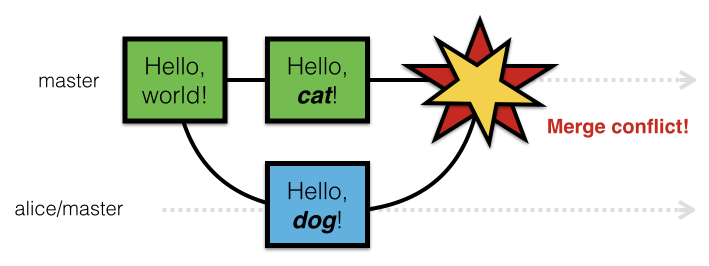
\includegraphics [scale=0.6]{step2}
%\caption{Sección de Issues}
\label{fig:issues}
\end{figure}
    
\end{block}
\end{frame}

%\section{Merge conflicts}

\begin{frame}{Merge conflicts or:}{How I Learned to Stop Worrying and Love my Code $\heartsuit$}

\begin{block}{Creamos nuevo repositorio}

\begin{figure}[h!]
\centering
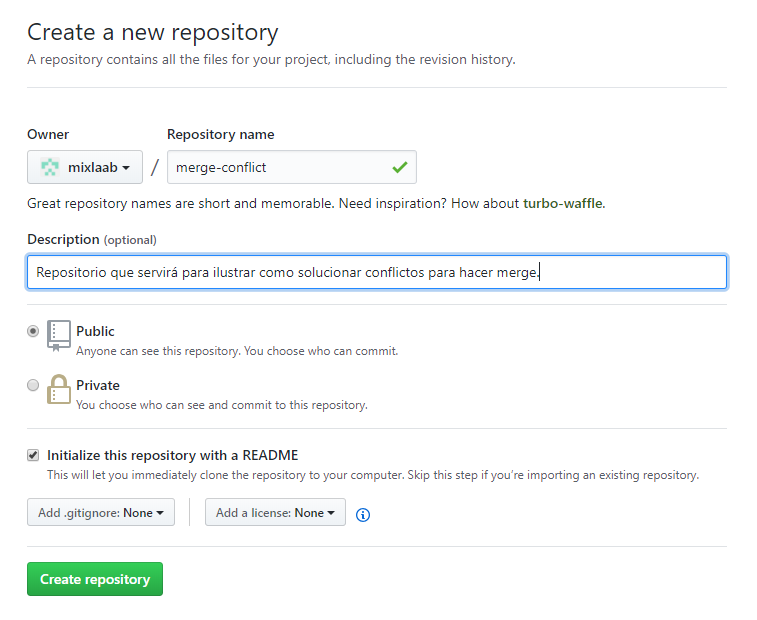
\includegraphics [scale=0.4]{newrepo}
%\caption{Sección de Issues}
\label{fig:issues}
\end{figure}
    
\end{block}

\end{frame}

\begin{frame}{Merge conflicts or:}{How I Learned to Stop Worrying and Love my Code $\heartsuit$}

\begin{block}{Página principal del 'repo'}

\begin{figure}[h!]
\centering
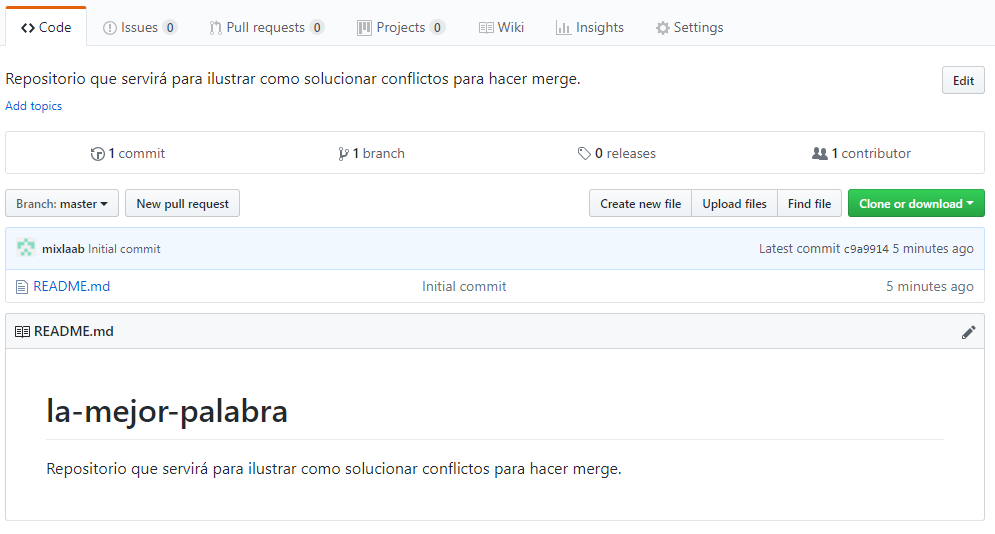
\includegraphics [scale=0.35]{pagprinc}
%\caption{Sección de Issues}
\label{fig:issues}
\end{figure}
    
\end{block}

\end{frame}

\begin{frame}{Merge conflicts or:}{How I Learned to Stop Worrying and Love my Code $\heartsuit$}

\begin{block}{La mejor palabra (Cuenta: mixlaab)}

\begin{figure}[h!]
\centering
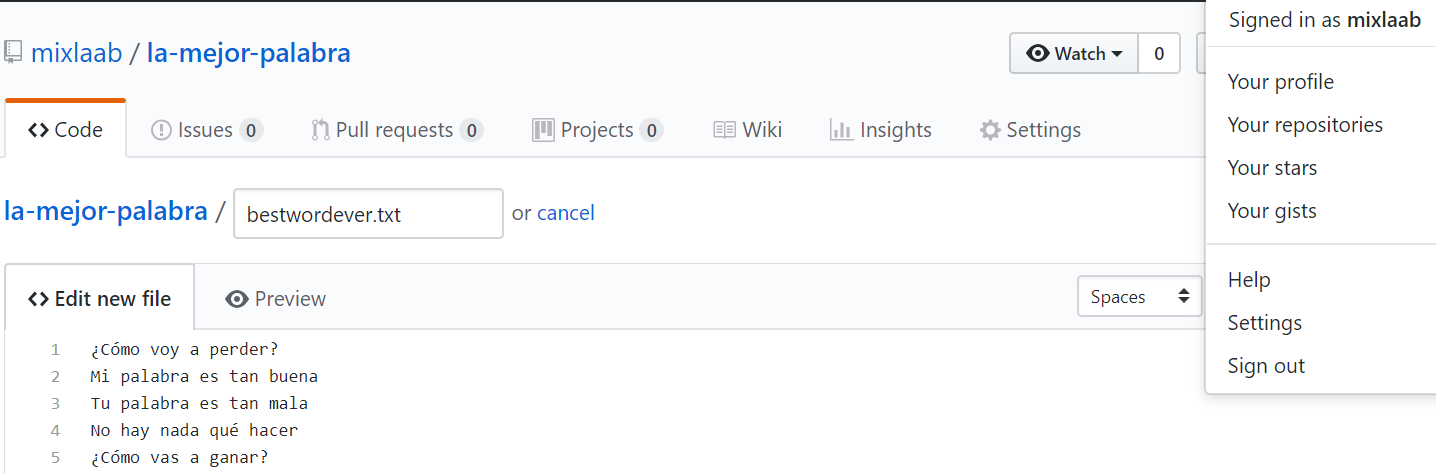
\includegraphics [scale=0.25]{bestwordever}
%\caption{Sección de Issues}
\label{fig:issues}
\end{figure}
    
\end{block}

\end{frame}

\begin{frame}{Merge conflicts or:}{How I Learned to Stop Worrying and Love my Code $\heartsuit$}

\begin{block}{La mejor palabra (Cuenta: mixlaab)}

\begin{figure}[h!]
\centering
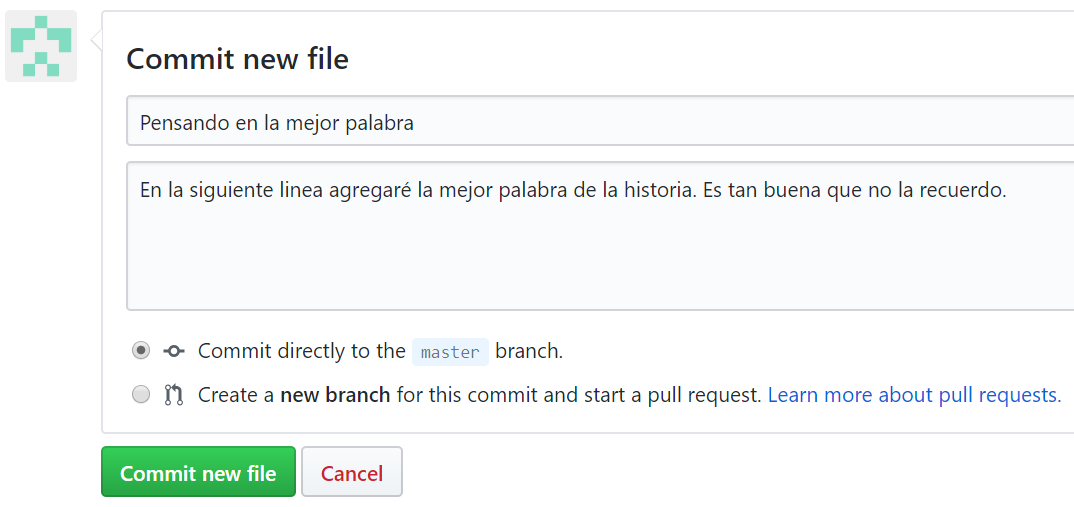
\includegraphics [scale=0.3]{bestwordever2}
%\caption{Sección de Issues}
\label{fig:issues}
\end{figure}
    
\end{block}

\end{frame}

\begin{frame}{Merge conflicts or:}{How I Learned to Stop Worrying and Love my Code $\heartsuit$}

\begin{block}{La mejor palabra (Cuenta: vdejesusmedrano)}

\begin{figure}[h!]
\centering
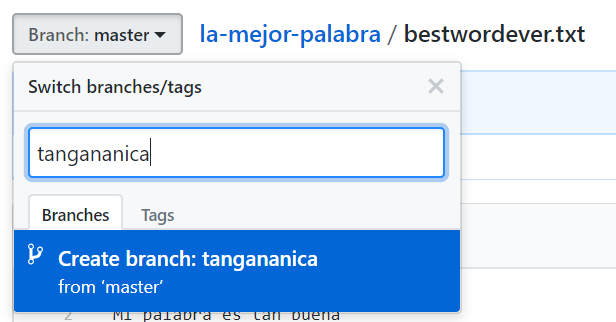
\includegraphics [scale=0.3]{tangananicabranch}
%\caption{Sección de Issues}
\label{fig:issues}
\end{figure}
    
\end{block}

\end{frame}

\begin{frame}{Merge conflicts or:}{How I Learned to Stop Worrying and Love my Code $\heartsuit$}

\begin{block}{La mejor palabra (Cuenta: vdejesusmedrano)}

\begin{figure}[h!]
\centering
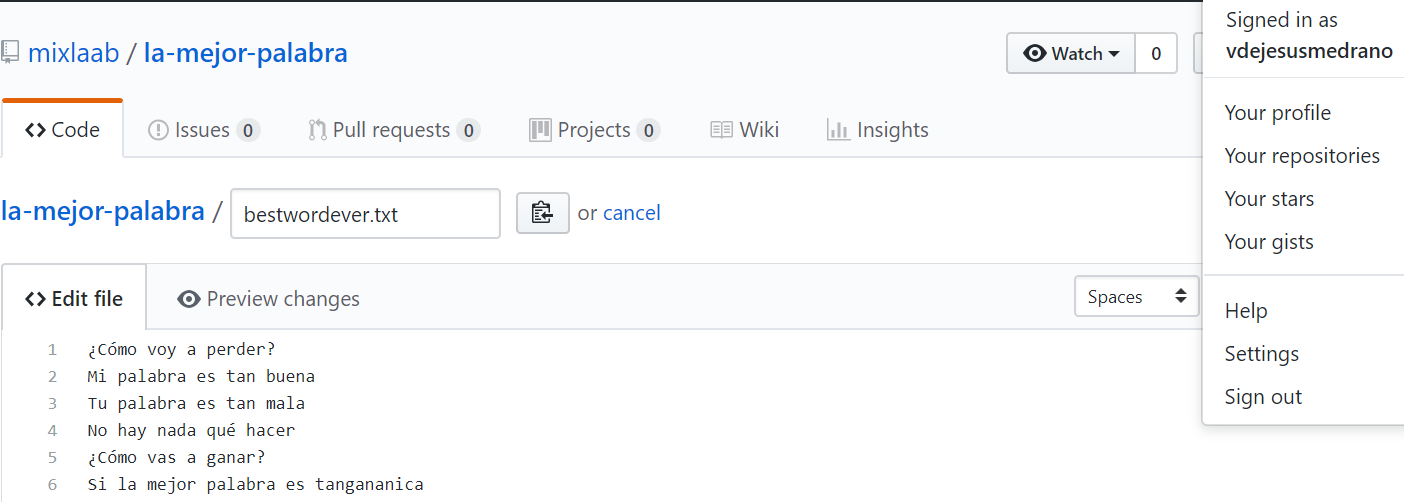
\includegraphics [scale=0.25]{tangananica}
%\caption{Sección de Issues}
\label{fig:issues}
\end{figure}
    
\end{block}

\end{frame}

\begin{frame}{Merge conflicts or:}{How I Learned to Stop Worrying and Love my Code $\heartsuit$}

\begin{block}{La mejor palabra (Cuenta: vdejesusmedrano)}

\begin{figure}[h!]
\centering
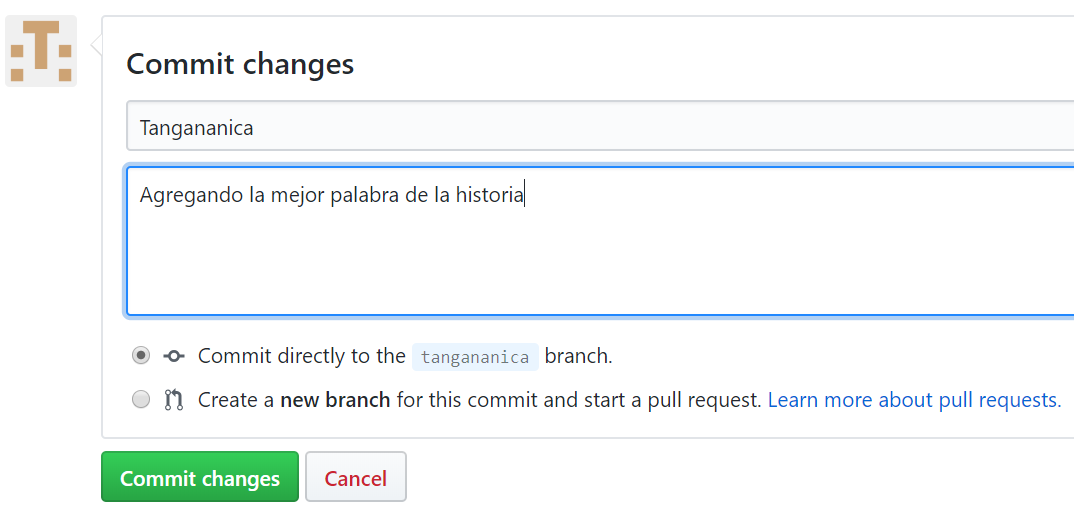
\includegraphics [scale=0.3]{tangananica2}
%\caption{Sección de Issues}
\label{fig:issues}
\end{figure}
    
\end{block}

\end{frame}

\begin{frame}{Merge conflicts or:}{How I Learned to Stop Worrying and Love my Code $\heartsuit$}

\begin{block}{La mejor palabra (Cuenta: mixlaab)}

\begin{figure}[h!]
\centering
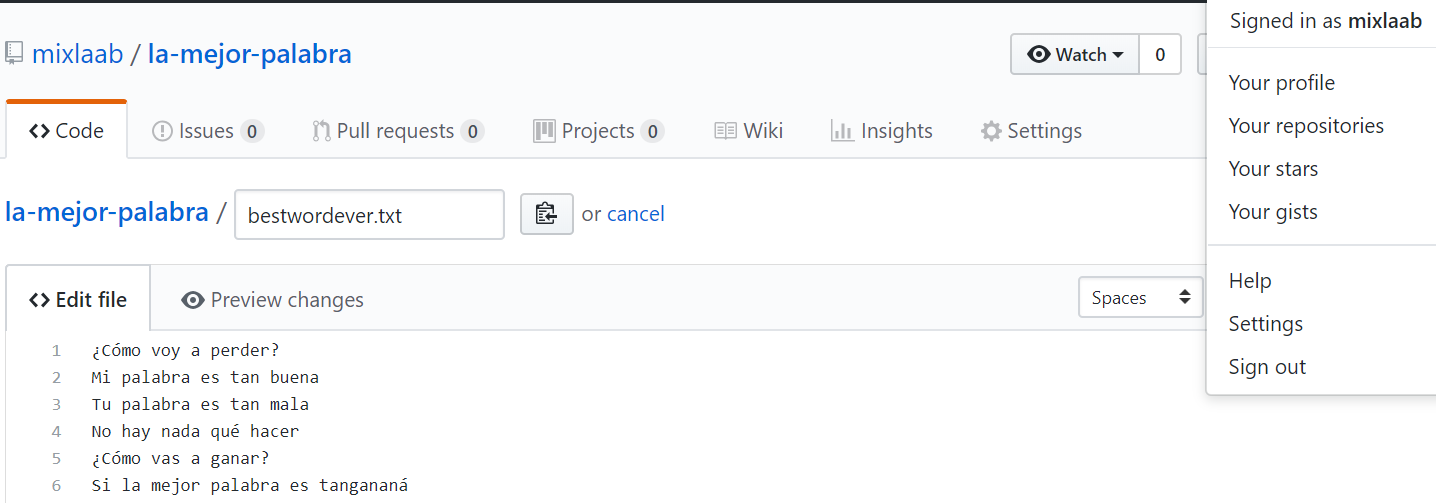
\includegraphics [scale=0.25]{tanganana}
%\caption{Sección de Issues}
\label{fig:issues}
\end{figure}
    
\end{block}

\end{frame}

\begin{frame}{Merge conflicts or:}{How I Learned to Stop Worrying and Love my Code $\heartsuit$}

\begin{block}{La mejor palabra (Cuenta: mixlaab)}

\begin{figure}[h!]
\centering
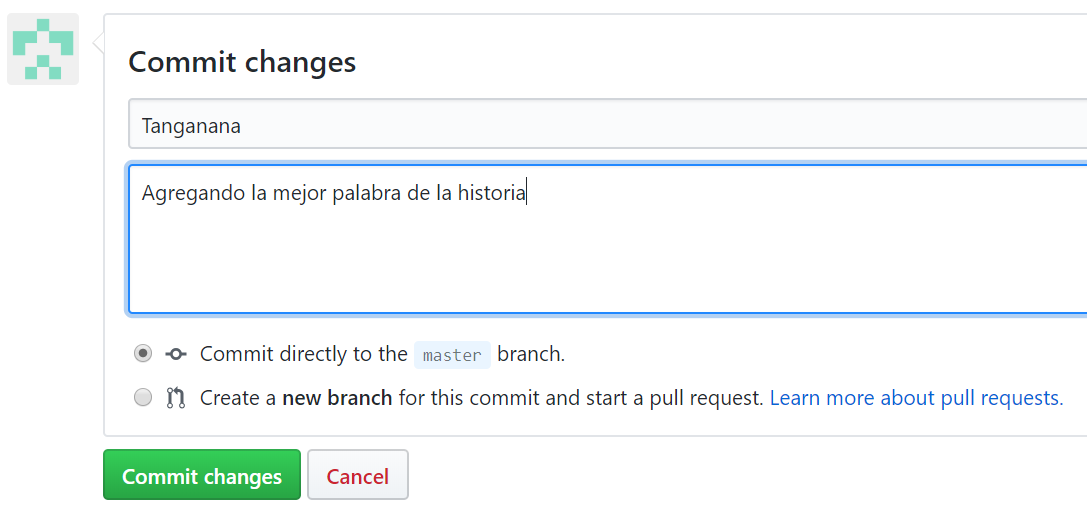
\includegraphics [scale=0.3]{tanganana2}
%\caption{Sección de Issues}
\label{fig:issues}
\end{figure}
    
\end{block}

\end{frame}

\begin{frame}{Merge conflicts or:}{How I Learned to Stop Worrying and Love my Code $\heartsuit$}

\begin{block}{Red del repositorio (Cuenta: mixlaab)}

\begin{figure}[h!]
\centering
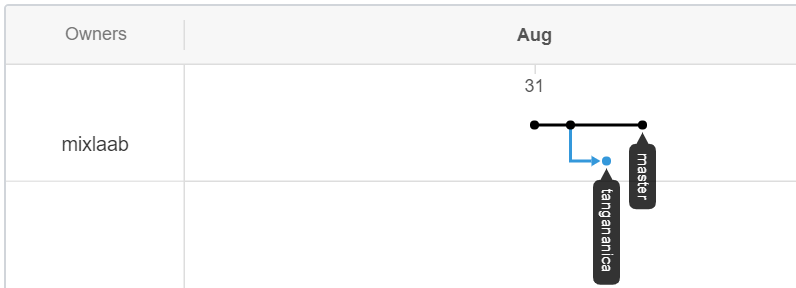
\includegraphics [scale=0.3]{network}
%\caption{Sección de Issues}
\label{fig:issues}
\end{figure}
    
\end{block}

\end{frame}

%\begin{frame}{Merge conflicts or:}{How I Learned to Stop Worrying and Love my Code \heartsuit}

%\begin{block}{Pull request (Cuenta: vdejesusmedrano)}

%\begin{figure}[h!]
%\centering
%
\includegraphics [scale=0.25]{pullrequest}
%\caption{Sección de Issues}
%\label{fig:issues}
%\end{figure}
    
%\end{block}

%\end{frame}

\begin{frame}{Merge conflicts or:}{How I Learned to Stop Worrying and Love my Code $\heartsuit$}

\begin{block}{Solución del conflicto (Cuenta: mixlaab)}

\begin{figure}[h!]
\centering
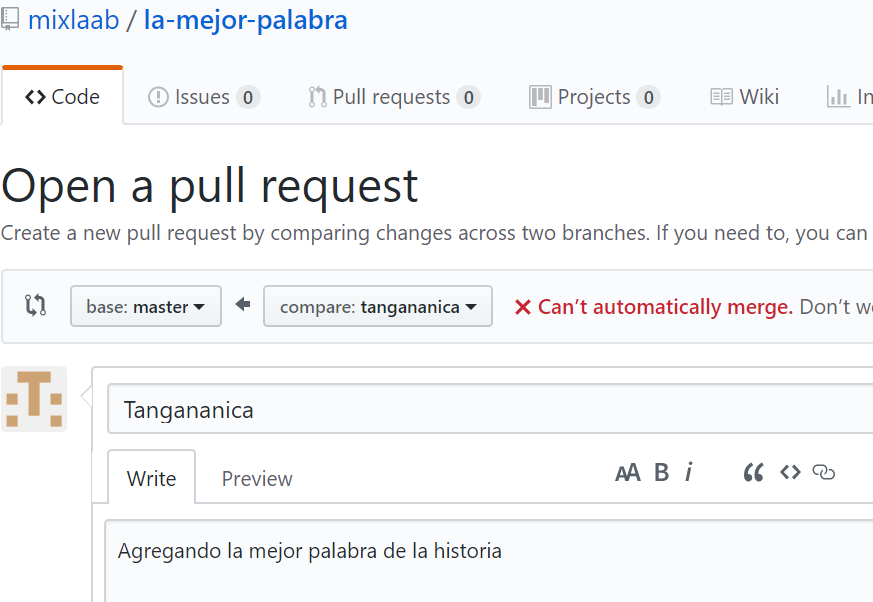
\includegraphics [scale=0.25]{conflict}
%\caption{Sección de Issues}
\label{fig:issues}
\end{figure}
    
\end{block}

\end{frame}

\begin{frame}{Merge conflicts or:}{How I Learned to Stop Worrying and Love my Code $\heartsuit$}

\begin{block}{Solución del conflicto (Cuenta: mixlaab)}

\begin{figure}[h!]
\centering
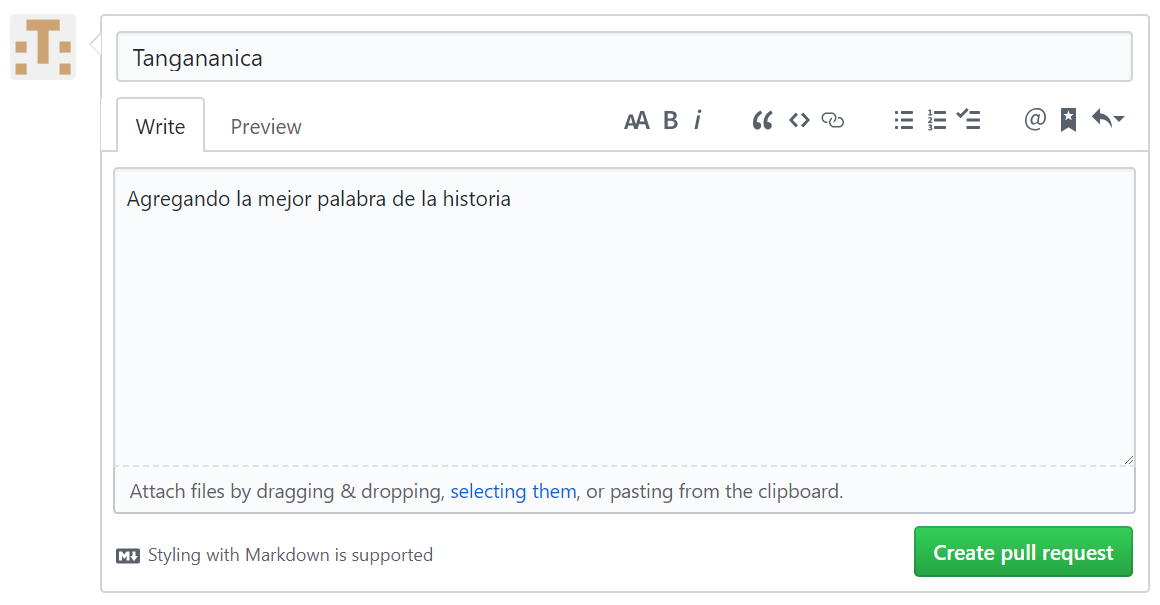
\includegraphics [scale=0.25]{conflict2}
%\caption{Sección de Issues}
\label{fig:issues}
\end{figure}
    
\end{block}

\end{frame}

\begin{frame}{Merge conflicts or:}{How I Learned to Stop Worrying and Love my Code $\heartsuit$}

\begin{block}{Solución del conflicto (Cuenta: mixlaab)}

\begin{figure}[h!]
\centering
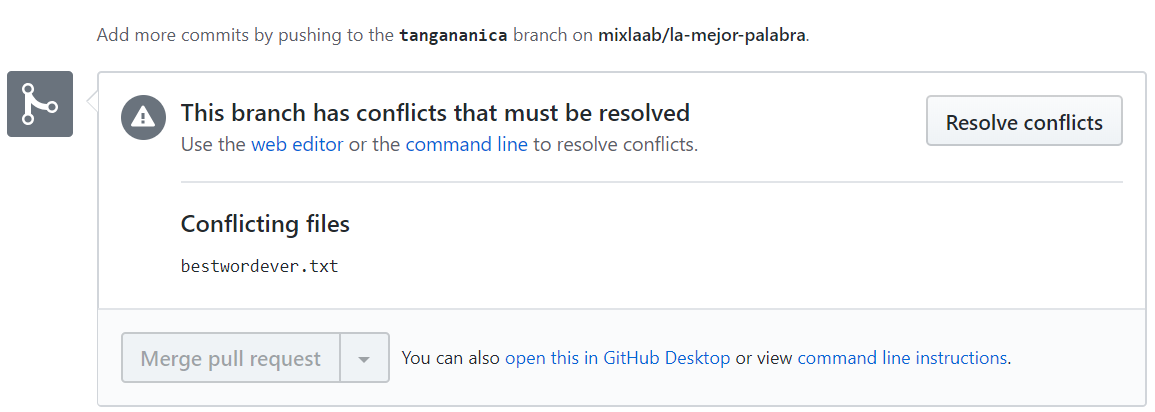
\includegraphics [scale=0.25]{conflict3}
%\caption{Sección de Issues}
\label{fig:issues}
\end{figure}
    
\end{block}

\end{frame}

\begin{frame}{Merge conflicts or:}{How I Learned to Stop Worrying and Love my Code $\heartsuit$}

\begin{block}{Solución del conflicto (Cuenta: mixlaab)}

\begin{figure}[h!]
\centering
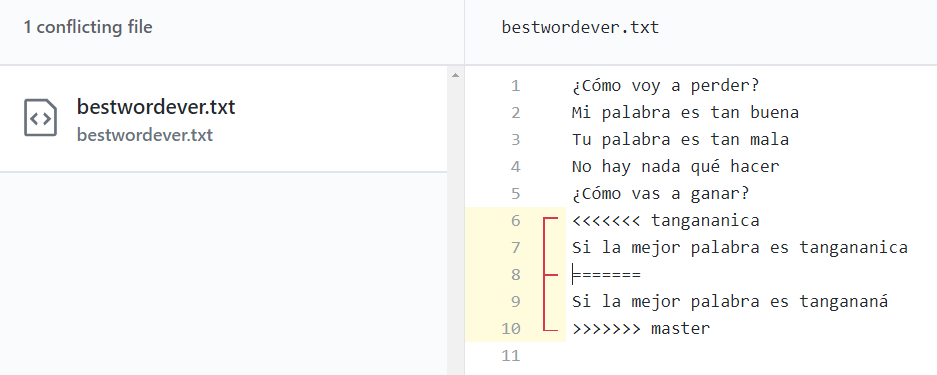
\includegraphics [scale=0.3]{conflict4}
%\caption{Sección de Issues}
\label{fig:issues}
\end{figure}
    
\end{block}

\end{frame}
\begin{frame}{Merge conflicts or:}{How I Learned to Stop Worrying and Love my Code $\heartsuit$}

\begin{block}{Solución del conflicto (Cuenta: mixlaab)}

\begin{columns}[c]
\column{1.9in}
%\vspace{0.2in}
\framebox{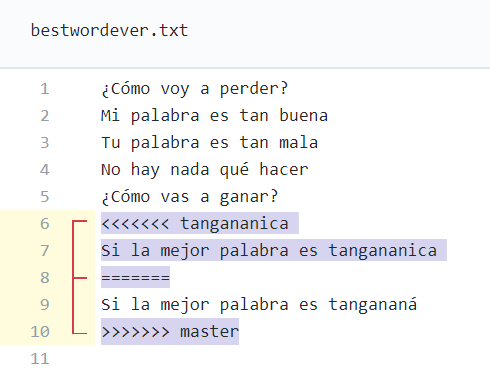
\includegraphics[width=1.9in]{conflict5}}

\column{1.3in}
\vspace{0.1in}
\framebox{
\includegraphics[width=1.3in]{conflict6}}
\end{columns}

    
\end{block}

\end{frame}

\begin{frame}{Merge conflicts or:}{How I Learned to Stop Worrying and Love my Code $\heartsuit$}

\begin{block}{Solución del conflicto (Cuenta: mixlaab)}

\begin{figure}[h!]
\centering
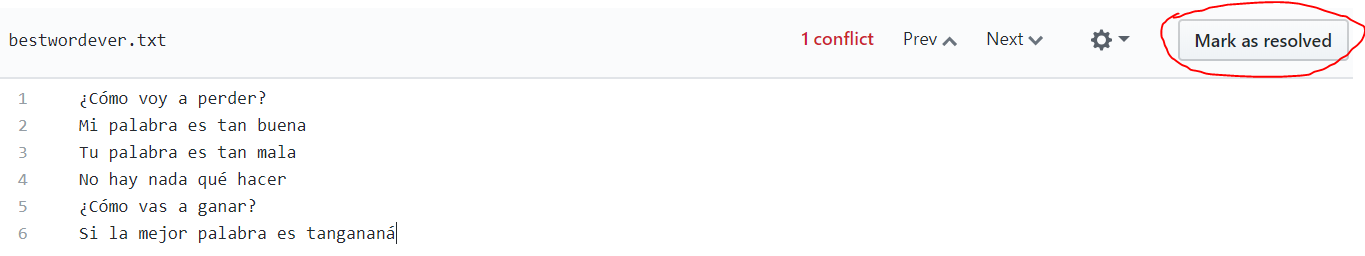
\includegraphics [scale=0.25]{conflict7}
%\caption{Sección de Issues}
\label{fig:issues}
\end{figure}
    
\end{block}

\end{frame}

\begin{frame}{Merge conflicts or:}{How I Learned to Stop Worrying and Love my Code $\heartsuit$}

\begin{block}{Solución del conflicto (Cuenta: mixlaab)}

\begin{figure}[h!]
\centering
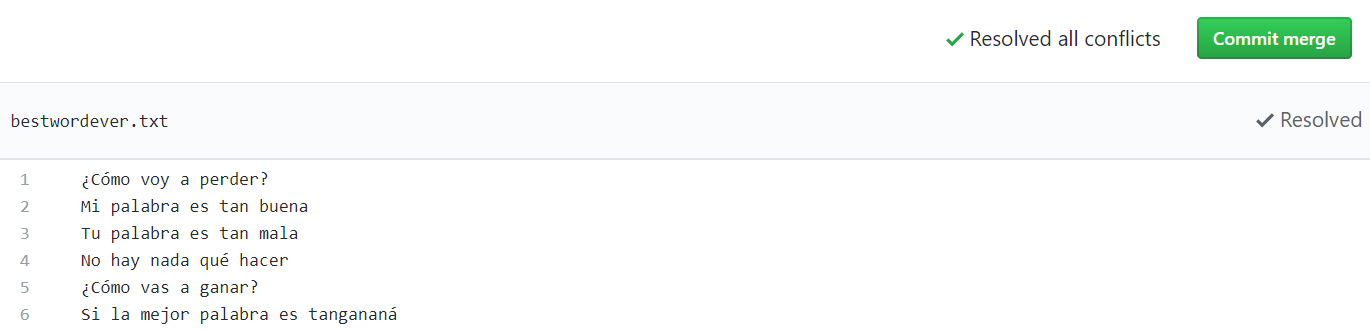
\includegraphics [scale=0.25]{conflict8}
%\caption{Sección de Issues}
\label{fig:issues}
\end{figure}
    
\end{block}

\end{frame}

\begin{frame}{Merge conflicts or:}{How I Learned to Stop Worrying and Love my Code $\heartsuit$}

\begin{block}{Solución del conflicto (Cuenta: mixlaab)}

\begin{figure}[h!]
\centering

\includegraphics [scale=0.25]{merge}
%\caption{Sección de Issues}
\label{fig:issues}
\end{figure}
    
\end{block}

\end{frame}

\begin{frame}{Merge conflicts or:}{How I Learned to Stop Worrying and Love my Code $\heartsuit$}

\begin{block}{Solución del conflicto (Cuenta: mixlaab)}

\begin{figure}[h!]
\centering

\includegraphics [scale=0.25]{merge2}
%\caption{Sección de Issues}
\label{fig:issues}
\end{figure}
    
\end{block}

\end{frame}

\begin{frame}{Merge conflicts or:}{How I Learned to Stop Worrying and Love my Code $\heartsuit$}

\begin{block}{Solución del conflicto (Cuenta: mixlaab)}

\begin{figure}[h!]
\centering

\includegraphics [scale=0.25]{merge3}
%\caption{Sección de Issues}
\label{fig:issues}
\end{figure}
    
\end{block}

\end{frame}

\begin{frame}{Merge conflicts or:}{How I Learned to Stop Worrying and Love my Code $\heartsuit$}

\begin{block}{Solución del conflicto (Cuenta: mixlaab)}

\begin{figure}[h!]
\centering
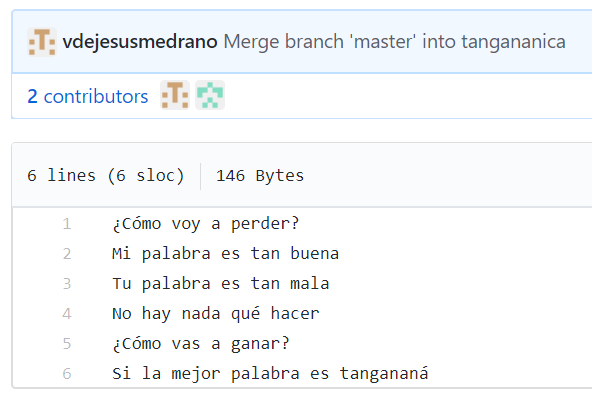
\includegraphics [scale=0.25]{final1}
%\caption{Sección de Issues}
\label{fig:issues}
\end{figure}
    
\end{block}

\end{frame}

\begin{frame}{Merge conflicts or:}{How I Learned to Stop Worrying and Love my Code $\heartsuit$}

\begin{block}{Solución del conflicto (Cuenta: mixlaab)}

\begin{figure}[h!]
\centering
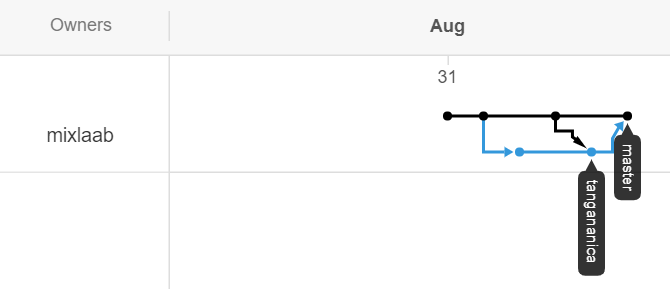
\includegraphics [scale=0.45]{final2}
%\caption{Sección de Issues}
\label{fig:issues}
\end{figure}
    
\end{block}

\end{frame}




\section{Información de contacto}
% contact information
\begin{frame}{Feedback}{Información de contacto}
En caso de comentarios, sugerencias, preguntas o errores en las diapositivas no dudes en contactarme.
  \begin{center}
    \insertauthor\\
    \chref{https://mixlaab.github.io}{https://mixlaab.github.io}\\
    WA: 8119022700\\
    %9220 Aalborg Ø
  \end{center}
\end{frame}
%%%%%%%%%%%%%%%%

{\aauwavesbg%
\begin{frame}[plain,noframenumbering]%
  \finalpage{Fin}
\end{frame}}
%%%%%%%%%%%%%%%%

\end{document}
